\documentclass[tikz,border=8pt]{standalone}
\usepackage{tikz}
\usepackage{pgfplots}
\usepackage{amsmath, amssymb}

\pgfplotsset{compat=1.18}

\begin{document}

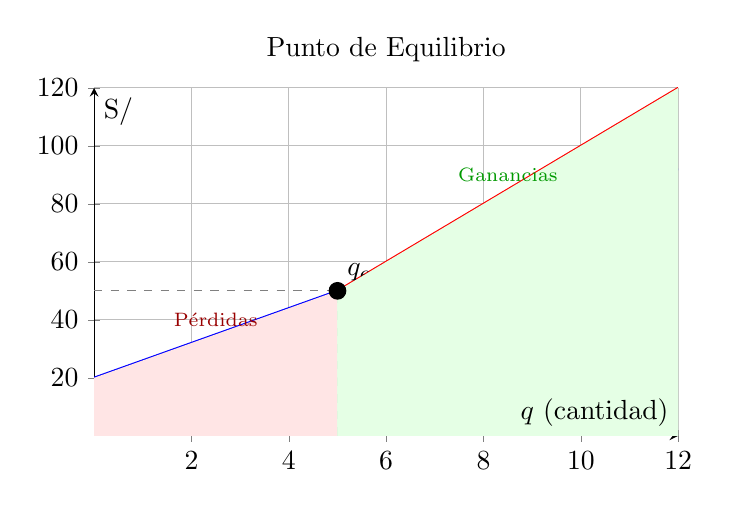
\begin{tikzpicture}[scale=1.0]

  % Gráfica del punto de equilibrio
  \begin{axis}[
    axis lines = middle,
    xlabel = {$q$ (cantidad)},
    ylabel = {S/},
    title = {Punto de Equilibrio},
    xmin = 0, xmax = 12,
    ymin = 0, ymax = 120,
    xtick = {0,2,4,6,8,10,12},
    ytick = {0,20,40,60,80,100,120},
    grid = major,
    width = 9cm,
    height = 6cm,
  ]

    % Recta de Costo Total: C_T(q) = 20 + 6q
    \addplot[blue, thick, domain=0:12, samples=100] {20 + 6*x};
    \node[blue, rotate=40] at (axis cs:9, 70) {$C_T(q)$};

    % Recta de Ingreso Total: I(q) = 10q
    \addplot[red, thick, domain=0:12, samples=100] {10*x};
    \node[red, rotate=55] at (axis cs:7, 60) {$I(q)$};

    % Punto de equilibrio: q_e = 5, I_e = 50
    \addplot[only marks, mark=*, mark size=3pt, black] coordinates {(5,50)};
    \node[black, above right] at (axis cs:5,50) {$q_e = 5$};

    % Líneas guía al punto de equilibrio
    \addplot[dashed, gray] coordinates {(5,0) (5,50)};
    \addplot[dashed, gray] coordinates {(0,50) (5,50)};

    % Zona de pérdidas (sombreado entre las dos rectas de 0 a 5)
    \addplot[draw=none, fill=red!10, domain=0:5, samples=100] {20+6*x} \closedcycle;
    \addplot[draw=none, fill=red!10, domain=0:5, samples=100] {10*x} \closedcycle;

    % Zona de ganancias (sombreado entre las dos rectas de 5 a 12)
    \addplot[draw=none, fill=green!10, domain=5:12, samples=100] {20+6*x} \closedcycle;
    \addplot[draw=none, fill=green!10, domain=5:12, samples=100] {10*x} \closedcycle;

    \node[red!60!black, font=\scriptsize] at (axis cs:2.5, 40) {Pérdidas};
    \node[green!60!black, font=\scriptsize] at (axis cs:8.5, 90) {Ganancias};

  \end{axis}

\end{tikzpicture}

\end{document}
